\chapter{康托尔集合论:无穷的性质}

\section{无穷集合的比较}
\subsection{引入}
想必大家一定听说过有名的无限旅馆的故事.

\paragraph{希尔伯特旅馆}
有一家无限间房间的旅馆, 但旅馆已经满客.
此时来了一位客人想要入住, 老板说:“没问题!”
老板安排1号房客人挪到2号房, 2号房挪到3号房, 3号房挪到4号房, 以此类推.
结果是1号房空出来了, 新客人可以入住了.
而这时又来了无穷多的客人, 老板又说:“没问题!”
然后老板发布通知, 每个客人都挪到自己房间号两倍的房间, 这样奇数号房间都空出来了, 无穷多的客人可以入住了.

这个故事看似荒诞不经, 但并非毫无道理, 其与无穷集合的比较有关.

\subsection{定义}
\label{defi}
假设我们并不认识$3$以上的数字, 那么我们要怎么比较$7$枚铜币和$8$枚铁币呢?
其实我们可以将铜币和铁币一个一个拿出, 每次各拿一个, 最后剩下哪一种币, 就是哪一种数量多.
同样, 我们可以用这种方法比较无穷集合的大小, 如偶数集与奇数集的元素个数一样多:
\begin{table}[!ht]
  \centering
    \begin{tabular}{c|lllll}
      \toprule
      $\mathrm O$ & 1 & 3 & 5 & 7 & $\cdots$ \\
      \midrule
      $\mathrm E$ & 2 & 4 & 6 & 8 & $\cdots$ \\
      \bottomrule
    \end{tabular}
    \caption{奇数与偶数一一对应}
\end{table}

虽然可能有点颠覆认知, 但是通过这种方法, 我们得出了正整数集与偶数集一样大的结论.

\begin{table}[!h]
  \centering
    \begin{tabular}{c|lllll}
      \toprule
      $\mathrm N_+$ & 1 & 2 & 3 & 4 & $\cdots$ \\
      \midrule
      $\mathrm O$   & 2 & 4 & 6 & 8 & $\cdots$ \\
      \bottomrule
    \end{tabular}
    \caption{正整数与偶数一一对应}
\end{table}

同样, 正平方数集与正整数集一样大.

\begin{table}[!h]
  \centering
    \begin{tabular}{c|lllll}
      \toprule
      $\mathrm N_+$ & 1 & 2 & 3 & 4  & $\cdots$ \\
      \midrule
      $n^2$         & 1 & 4 & 9 & 16 & $\cdots$ \\
      \bottomrule
    \end{tabular}
    \caption{奇数与偶数一一对应}
\end{table}

那如果两个无穷集合无法一一对应, 那如何比较谁大谁小呢?

\begin{definition}
  若集合$A$与$B$无法建立一一对应, 且$B$的一个子集为$C$(同样也是无穷集合), $C$能够与$A$建立一一对应关系, 则$B$比$A$大.
  记为$\abs{B} > \abs{A}$.
\end{definition}

\section{正整数集与有理数}

了解以上定义之后, 我们是时候研究一下各无穷集合之间的关系了,
那我们先来会会我们的老朋友正整数集$\mathbb N_+$与有理数集$\mathbb Q$.
有理数集看似远远大于正整数集, 但是不要被表象迷惑, 他们俩之间存在一种巧妙的对应关系.

\begin{figure}[htbp]
  \centering
    \documentclass[border=10pt, tikz]{standalone}
\usepackage{amsmath}
\usepackage{amssymb}
\usepackage{ctex}
\usepackage{xcolor}
\usepackage{tikz}
\usetikzlibrary{matrix, calc, positioning}
\usetikzlibrary{arrows.meta}

\begin{document}
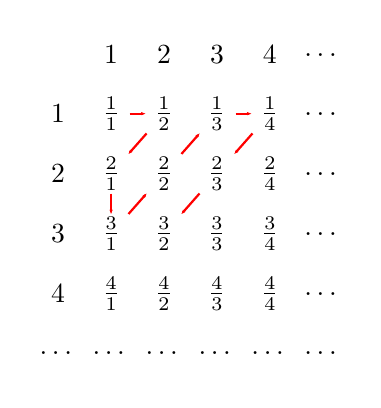
\begin{tikzpicture}
	% 定义矩阵
	\matrix (m) [matrix of nodes, nodes={minimum size=1.3em, inner sep=1pt, anchor=center},
		column sep=-0.5\pgflinewidth+4pt, row sep=-0.5\pgflinewidth+8pt]
	{
		~      & 1             & 2             & 3             & 4             & \ldots \\
		1      & $\frac{1}{1}$ & $\frac{1}{2}$ & $\frac{1}{3}$ & $\frac{1}{4}$ & \ldots \\
		2      & $\frac{2}{1}$ & $\frac{2}{2}$ & $\frac{2}{3}$ & $\frac{2}{4}$ & \ldots \\
		3      & $\frac{3}{1}$ & $\frac{3}{2}$ & $\frac{3}{3}$ & $\frac{3}{4}$ & \ldots \\
		4      & $\frac{4}{1}$ & $\frac{4}{2}$ & $\frac{4}{3}$ & $\frac{4}{4}$ & \ldots \\
		\ldots & \ldots        & \ldots        & \ldots        & \ldots        & \ldots \\
	};

	% 绘制折线
	\tikzset{
	arrow/.style = {arrows = {-Stealth[length=3pt, inset=2pt]}, thick, red}
	}

	\draw (m-2-2) edge [arrow] (m-2-3);
	\draw (m-2-3) edge [arrow] (m-3-2);
	\draw (m-3-2) edge [arrow] (m-4-2);
	\draw (m-4-2) edge [arrow] (m-3-3);
	\draw (m-3-3) edge [arrow] (m-2-4);
	\draw (m-2-4) edge [arrow] (m-2-5);
	\draw (m-2-5) edge [arrow] (m-3-4);
	\draw (m-3-4) edge [arrow] (m-4-3);

\end{tikzpicture}
\end{document}

    \caption{自然数与有理数的一一对应}
    \label{fig:bijection}
\end{figure}

如 \cref{fig:bijection}, 我们制出一个关于有正有理数的表, 我们可以肯定里面肯定包括了所有的正有理数,
按照红线将其拉长成1条直线, 再去掉重复的项,
我们就得到了一个正有理数的集合, 可以用这样的排列方法将有理数与正整数一一对应.
\footnote{编者按:即有理数集是可数集. }

但是这个集合只是与正有理数等大, 而不是与有理数等大.
所以我们要运用无限旅馆中的技巧.
我们将正整数分为三部分:

\begin{enumerate}
  \item \label{enum:1} ${1}$
  \item \label{enum:2} 偶数
  \item \label{enum:3} 除$1$以外的偶数
\end{enumerate}

将\cref{enum:1}与$0$对应,
将\cref{enum:2}与新的正整数$\mathbb N_+$对应,
再按如上方法与正有理数对应.
如下:

\begin{table}[h!]
  \centering
    \begin{tabular}{c|lllll}
      \toprule
      $\mathrm N_+$ & 1 & 2             & 3 & 4 & $\cdots$ \\
      \midrule
      $\mathrm O$   & 2 & 4             & 6 & 8 & $\cdots$ \\
      \midrule
      $\mathrm Q_+$ & 1 & $\frac{1}{2}$ & 2 & 3 & $\cdots$ \\
      \bottomrule
    \end{tabular}
    \caption{间接对应}
\end{table}

而\cref{enum:3}也一样, 先与一个新的整数集\footnote{编者注:此处应该为奇数集}对应, 再与负有理数集$\mathbb Q_-$对应.
这样正整数集的三部分就分别对应了有理数的$0$、正、负三部分, 我们得到了正整数与有理数等大的结论.

\subsection{幂集}
\label{ssec:powerset}
我们在 \cref{defi} 中说到,
无法互相一一对应的无穷集合, 可能会有人质疑存在这样的集合吗?
其实, 这一方面的奠基人康托尔
\footnote{编者注: Cantor,Georg Ferdinand Ludwig Philipp,
  1845年3月3日--1918年1月6日.
集合论的创始人, 最早从事无穷集合的一般理论研究的数学家. }
已经为我们发明了一种工具:幂集.

\begin{definition}[幂集(power set)]
  给定集合$A$ , 记$2^{A}$为集合 $A$  的子集的集合, 即 $2^{A}=\{ X|X\subset A \}$. 称
  $2^{A}$ 是 $A$ 的\textbf{幂集(power set)}.
  \footnote{编者注:这里不同于原文, 采用了一种更加常见的记法. },
\end{definition}

如果$A=\{1, 2, 3\}$ , 那么就有
\[
  2^A=\{\varnothing, \{1\}, \{2\}, \{3\}, \{1, 2\}, \{1, 3\}, \{2, 3\}, A\}
.\]
注意空集 $\varnothing$ 和 $A$本身都是 $2^{A}$ 的元素, 取子集的时候不要忘了空集和集合本身.
\footnote{由于无穷集合的幂集难以用列举法表示此处用有限集来举例. }

集合和幂集的基数之间有什么关系呢?

答案是 $\abs{2^A} =2^{ \abs{A} }$, 这也是把幂集记为 $2^A$ 的主要原因.
对于有限集合 $A$, 显然有 $\abs{2^A} =2^{ \abs{A} }> \abs{A}$,
那么对于无限集合 $B$ 会怎样呢?都是无限, $\abs{B}$ 和 $\abs{2^B}$ 相等吗?

答案是否定的, 因为不存在 $B$ 到 $2^B$ 的一一对应\footnote{编者注:此处应为满射. 如果 $f: A \to B$
中每个 $B$ 中元素都至少被$A$中的一个元素所对应, 那么称 $f$ 是一个\textbf{满射(surjection)}. },
按照定义, 这就是说, $\abs{2^B}$ 严格大于 $\abs{B}$.

\begin{proof}
  设$A= \{a,b,c,d,\cdots\}$($A$中的元素不局限于数字).
  假设$A$与$2^{A}$存在对应关系.
  例如:
  \begin{table}
    \centering

      \begin{tabular}{ccc}
        \toprule
        $A$      & ~                 & $2^{A}$                  \\
        \midrule
        $a$      & $\leftrightarrow$ & $\{a,\theta ,\varphi \}$ \\
        $b$      & $\leftrightarrow$ & $\varnothing$            \\
        $c$      & $\leftrightarrow$ & $\{m,n,o \ldots \}$      \\
        $\ldots$ & $\leftrightarrow$ & $\ldots$                 \\
        \bottomrule
      \end{tabular}
      \caption{元素与其幂集的子集的对应关系}

  \end{table}
  则发现, 左边$A$中的元素可分为两类:
  \begin{enumerate}
    \item \label{enum:in}属于其右边对应的集合(A的子集之一)
    \item \label{enum:notin}不属于其右边对应的集合
  \end{enumerate}
  那么\cref{enum:notin}中的元素就可以构成一个集合.
  设为集合$T$. 因为$T\subset A$, $T \in 2^{A} $.
  所以$T$也有一个对应的$A$中的元素, 设为$t$.

  所以
  \begin{enumerate}
    \item 若$t \in T$, 则 $t$ 是 \cref{enum:in} 所指的元素, 而 \cref{enum:in}
      的元素并没有被归入 $T$, 所以 $t \not\in T$, 矛盾.
    \item 若$t \not\in T$, 则 $t$ 是 \cref{enum:notin} 所指的元素, 所以 $t$
      被归入了 集合$T$, 得到 $t \in T$, 矛盾.
  \end{enumerate}

  结果就是, 无论以哪种方法对应, 总存在这样的集合$T$, 使得没有$A$中的元素与其一一对应.
  所以$A$与$2^{A}$无法一一对应.
  但是$2^{A} $的子集能与$A$对应. (不妨取这样的子集$ \{ \{a\},\{b\},\{c\}, \ldots \}
  $显然能与$A = \{a, b, c, d, \ldots \} $一一对应).

  所以$\abs{2^{A}}> \abs{A}$.

\end{proof}

\subsection{
  \texorpdfstring{$\left[ 0, 1 \right]$与$2^{\mathbb{N}_+}
  $与$\mathbb{R}$上的任意点}{[0, 1]与2\^N+与R上的任意点}
}
在我们证明完 $2^{A}>A$之后, 我们想到:$2^{\mathbb{N}_+} $太难理解了,
有没有什么直观的集合跟他等势
\footnote{我们把集合所包含的元素数量称作\textbf{基数}(cardinal, 或\textbf{势}).
用这个术语来说, 比较集合的大小就是在比较它们的基数的大小. }
呢.

有的兄弟, 有的. 就是$\left[0, 1\right]$.

\begin{note}[任意进制的数字表述] \label{note:system_of_numeration}
  在任意进制的数字表示中,
  小数点前第$n$位表示的是该进制基数的$n-1$次方,
  小数点后第$n$位表示的是该进制基数的$-n$次方.

  例如: 在十进制的$123. 4$中, 个位数的3表示$3 \times 10^{0} $,
  十位数的2表示$2 \times 10^{1} $,
  百位数的1表示$1 \times 10^{2} $,
  而十分位数的4表示$4 \times 10^{-1} $.

  我们将n进制数标记为右上角的「$^{(n)}$」, 例如我们将二进制数$11010$记为$11010^{(2)}$
\end{note}

让我们将$\left[ 0, 1 \right]$中的小数记为二进制.
不妨记 $1^{(10)} $ 为$0. 1111\ldots ^{(2)} $
记$0^{(10)} $为 $0. 0000\ldots ^{(2)} $.

\begin{note}[$0. 1111\ldots ^{(2)}  $等于$1^{(10)}$]
  由\cref{note:system_of_numeration}我们得知
  \begin{align*}
    0. 1111\ldots ^{(2)} & = \sum_{n=1}^{\infty} \frac{1}{2^{-n}}          \\
    & = \frac{1}{2}+\frac{1}{4} +\frac{1}{8} + \ldots \\
    & = 1
  \end{align*}
  不妨类比为$0. 999\ldots ^{(10)} = 1 ^{(10)} $
\end{note}

因为$2^{\mathbb{N}_+} $的元素是正整数构成的集合或者$\varnothing$,
我们不妨构造这样一个对应关系:属于$\left[0, 1\right]$的二进制小数, 若小数点后第$n$位是$1$,
则我们将$n$放入其对应的集合, 若为零则反之.

\begin{table}
  \centering
    \begin{tabular}{lcc}
      \toprule
      $0. 0000\ldots $               & $\leftrightarrow$ &
      $\varnothing$                                                 \\
      $0. 01101$                     & $\leftrightarrow$ & $\{2, 3,
      5\}$                                                          \\
      $0. 101100111000\ldots $ (无理数) & $\leftrightarrow$ & $\{1, 3,
      4, 7, 8, 9,\ldots \}  $                                       \\
      $0. 1111\ldots $               & $\leftrightarrow$ &
      $\mathbb{N}_+$                                                \\
      \bottomrule
    \end{tabular}
    \caption{[0, 1]的小数与自然数幂集的子集的对应关系}
    \label{tbl:01to2N}
\end{table}

\begin{figure}
  \centering
    \documentclass[border=3pt]{standalone}
\usepackage{tikz}
\usepackage{amsmath}
\usepackage{amssymb}
\usepackage{ctex}
\usetikzlibrary{matrix, calc, positioning}
\usepackage{pgfplots}
\pgfplotsset{compat=1.18}

\begin{document}

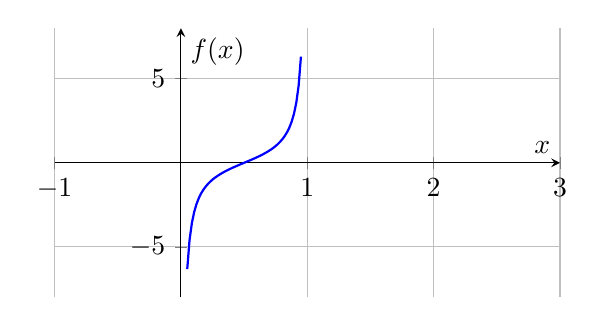
\begin{tikzpicture}
	\begin{axis}[
			axis lines = middle,
			xlabel = {\(x\)},
			ylabel = {\(f(x)\)},
			ymin=-8, ymax=8, % 设置 y 轴的范围
			xmin=-1, xmax=3, % 设置 x 轴的范围
			domain=0.05:0.95, % 设置函数的定义域
			samples=50, % 设置采样点数
			grid=both, % 显示网格
			width=8cm, % 设置图像的宽度
			height=5cm, % 设置图像的高度
		]
		\addplot [thick, blue] {tan(deg(pi*x - pi/2))}; % 绘制函数图像
	\end{axis}
\end{tikzpicture}

\end{document}

    \caption{函数图像} \label{fig:tan}
\end{figure}

例如 \cref{tbl:01to2N},
我们得到了$\left[0, 1\right]$与$2^{\mathbb{N}_+} $ 等势的结论.

我们又有一个明确的函数, 使$\left(0, 1\right)$与$\mathbb{R}$ 一一对应, 如\cref{fig:tan}
\begin{align}
  f \colon (0, 1) \to \mathbb{R} \colon f(x) = \tan (\pi x -
  \frac{\pi}{2}) \label{fn:tan01toR}
\end{align}

再运用无限旅馆的小技巧, 则有
\[
  2^{\mathbb{N}_+}\leftrightarrow [0, 1] \leftrightarrow (0, 1)
  \leftrightarrow \mathbb{R}
.\]

Amazing! $\abs{2^{\mathbb{N}_+}} = \abs{R}$ !

我们还能证明他们与平面上所有的点的集合$\mathbb{R}^{2} = \{(x,y)| x, y \in R\} $等势.

\begin{proof}

  取任意 $x \in (0, 1)$, 分离$x$的奇数位与偶数位, 按照原来的顺序排成两个新的小数,
  不妨让奇数位组成的小数为横坐标, 偶数位为纵坐标, 组成有序数对.

  例如:
  \[
    0. 114514 \leftrightarrow (0. 141, 0. 154)
  .\]
  从\cref{fn:tan01toR}我们可以构造函数 $g(a,b)$:
  \[
    g \colon \{(a,b) | a, b \in (0, 1) \}  \to \mathbb{R}^{2}  \colon
    g(a,b) = (f(a), f(b))
  .\]
  所以有
  \[
    [0, 1] \leftrightarrow \{(a,b)| a,b \in [0, 1]\} \leftrightarrow
    \mathbb{R}^{2}
  .\]
  所以任意二维有序数对(向量)所组成的集合与$2^{\mathbb{N}_+} $ 等势.
\end{proof}

同样地, 我们可以证明任意$n$维有序数对的集合与$2^{\mathbb{N}_+} $等势. 读者自证不难.

\subsection{\texorpdfstring{$\aleph $: Aleph 基数}{Aleph 基数}}

在\cref{ssec:powerset}中, 我们知道了一个无穷集的幂集一定大于这个无穷集自身. 所以这世上没有最大的集合, 只有更大的.
就像我们可以给实数排序一样, 我们也可以给无穷集按照基数大小排序.

我们用希伯来字母$\aleph$ (Aleph, 阿列夫) 来表示无穷大, 用下标表示级别. $\aleph_0 = \abs{\mathbb{N}}$
$\aleph_1 = \abs{\mathbb{R}}$.

\begin{definition}[无穷基数]
  若$\aleph_n =\abs{A}$, 那么 $\aleph_{n+1} = \abs{2^{A} }$
\end{definition}

\subsection{连续统假设}

\paragraph{连续统猜想(Continuum Hypothesis)}
康托尔研究集合论时提出
在可列集基数$\aleph_0$和实数基数$\aleph_{1}$之间没有别的基数, 这就是著名的连续统假设. 它又被称为希尔伯特第一问题.

\begin{note}
  18世纪70年代, 康托尔在研究无穷集的势时,
  首次发现不同的无穷可以具有不同的基数.
  自然数集的势被记作$\aleph_{0}$, 而实数集的势, 称为“连续统”, 记作 $\aleph_{1}$.

  康托尔提出一个问题:是否存在一个集合, 其基数严格大于 $\aleph_{0}$ 而小于 $\aleph_{1}$?这就是连续统假设(CH).
  也就是$2^{\aleph_0}$是否等于$\aleph_0$的继承者(successor), $\aleph_1$.

  康托尔猜想了$2^{\aleph_0}=\aleph_1$, 这就是
  ---因为希尔伯特将其放在他于1900年发表的一些重要而尚未解决的问题
  \footnote{希尔伯特(David Hilbert, 1862年1月23日--1943年2月14日,
    在一些历史著作中, 他与阿基米德、牛顿和高斯等重要数学家齐名, 被誉为“数学王子”)
    在1900年将连续统假设列为他提出的23个重要的数学难题中的第一题,
  标志着这一问题地位的确立. 它触及数学最根本的基础:形式系统是否有能力决定所有陈述的真假. }
  中, 而变得十分著名的---
  连续统猜想.
  其答案是连续统猜想是无法被判定的(undecidable).
\end{note}

哥德尔
\footnote{库尔特·哥德尔(Kurt Gödel, 1906年4月28日—1978年1月14日),
美籍奥地利数学家、逻辑学家和哲学家, 是二十世纪最伟大的逻辑学家之一, 其最杰出的贡献是哥德尔不完全性定理. }
证明了公理系统的\textbf{不完备性}---每个数学系统都存在一些命题永远无法被证明真伪.
这被称为\textbf{哥德尔不完备定理}.

再由保罗·寇恩
\footnote{保罗·寇恩(Paul Joseph Cohen, 1934年4月2日---2007年3月23日), 美国数学家,
凭借连续统假设的独立性证明于1966年获得菲尔兹奖章. }
用力迫法证明了连续统假设的不可判定性.

\paragraph{习题}
证明无穷集合$A$与其有穷子集组成的集合等大, 即
\[
  \abs{A} = \abs{ \{ B| B \subset A, \abs{B} \in \mathbb{N} \}  }
.\]

% paragraph infty_hotel  (end)
